\documentclass[12pt]{beamer}
\usepackage{graphicx}
\usepackage{hyperref}
\usepackage{listings}
\usepackage{color}
\usetheme{Default}
\setbeamertemplate{itemize items}[circle]

\input{listings-glsl.prf}


\lstset{
    numberstyle=\tiny\color{gray},
    keywordstyle=\color{blue},
    commentstyle=\color{darkgray},
    stringstyle=\color{pink},
    tabsize=4,
    breaklines=true,
    breakatwhitespace=true
}

\graphicspath{ {./images/} }

\title{Fur rendering with shells, fins, and order-independent transparency}
\author{Odd-Erik Frantzen\\ \url{https://github.com/odderikf/fur_project} }
\begin{document}
    \maketitle
    \begin{frame}
        \frametitle{Results:}
        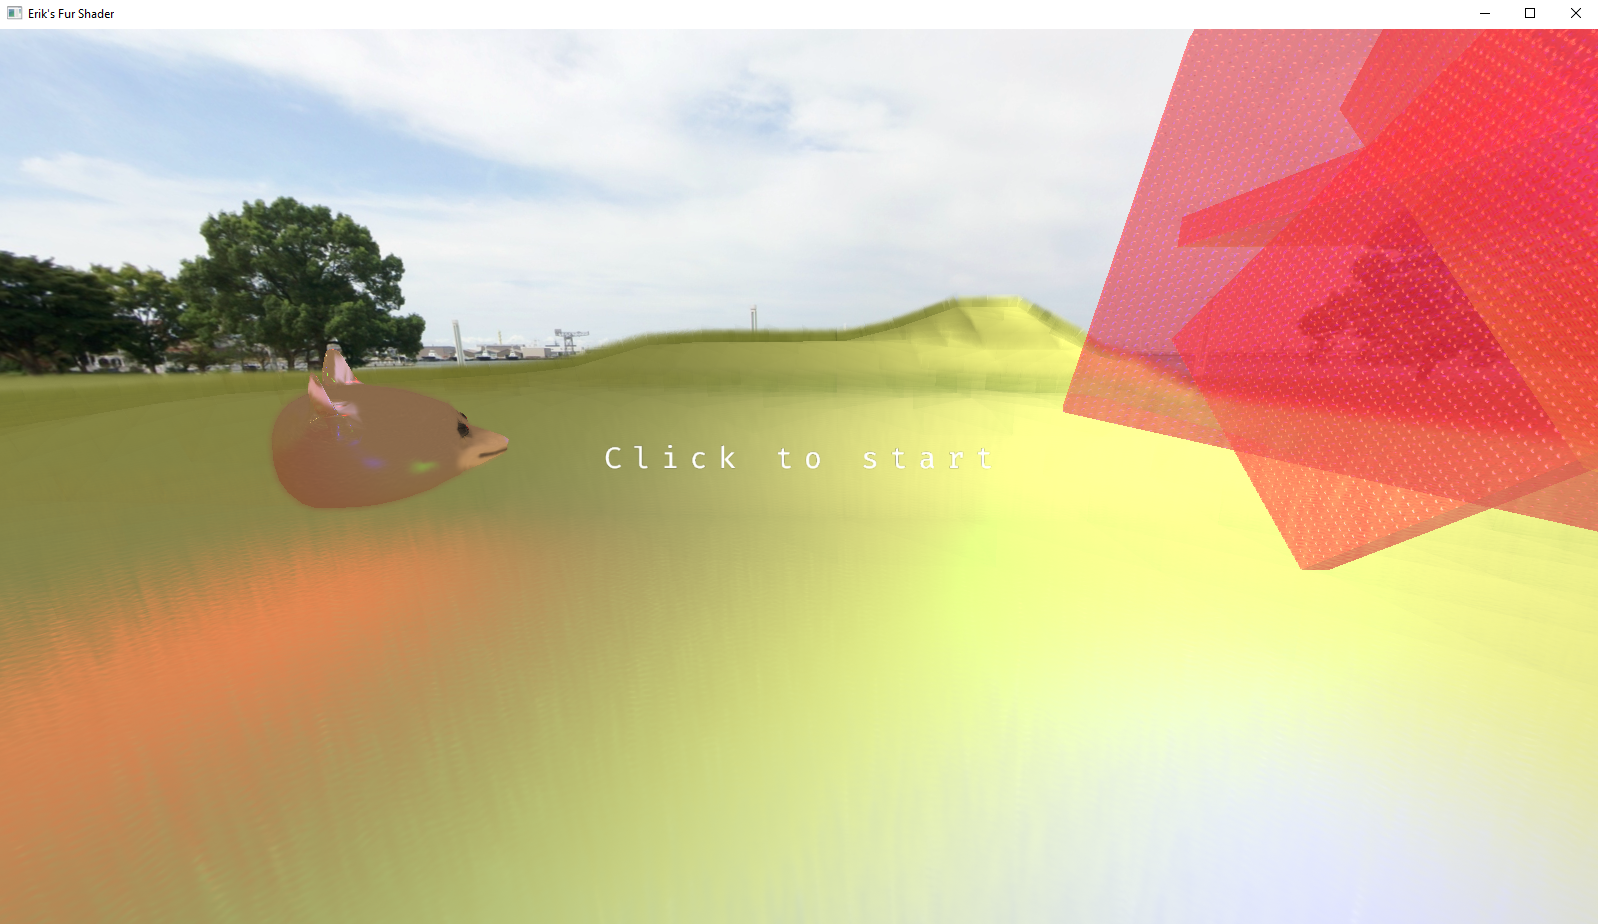
\includegraphics[width=\textwidth]{fullscene}
    \end{frame}
    \begin{frame}
        \frametitle{Results:}
        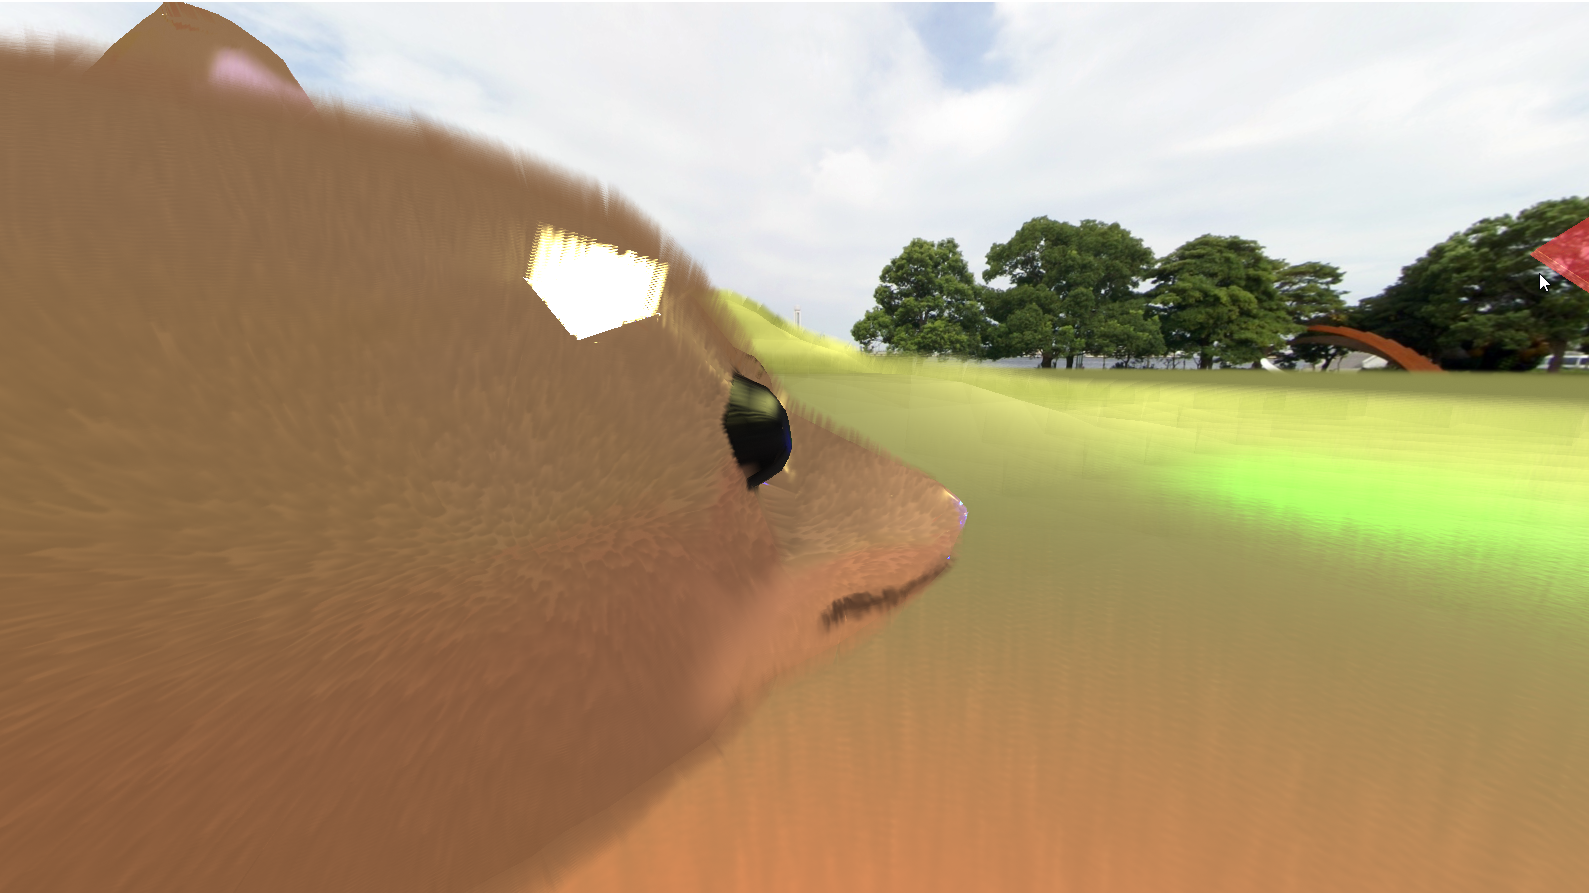
\includegraphics[width=\textwidth]{both}
    \end{frame}
    \begin{frame}
        \frametitle{Elements of the scene:}

        \begin{itemize}
            \item Things from previous exercises
            \begin{itemize}
                \item Phong lighting with dynamic pointlight sources
                \item Textured, normal mapped, roughness mapped objects.
            \end{itemize}

            \item Skybox at infinity
            \item Blender-exported object files and painted textures
            \item Shell-method fur volume generation
            \item Fin-method fur-card generation for better silhouettes
            \item Blending shader for semitransparent elements
        \end{itemize}
    \end{frame}
    \begin{frame}
        \frametitle{Skybox}
        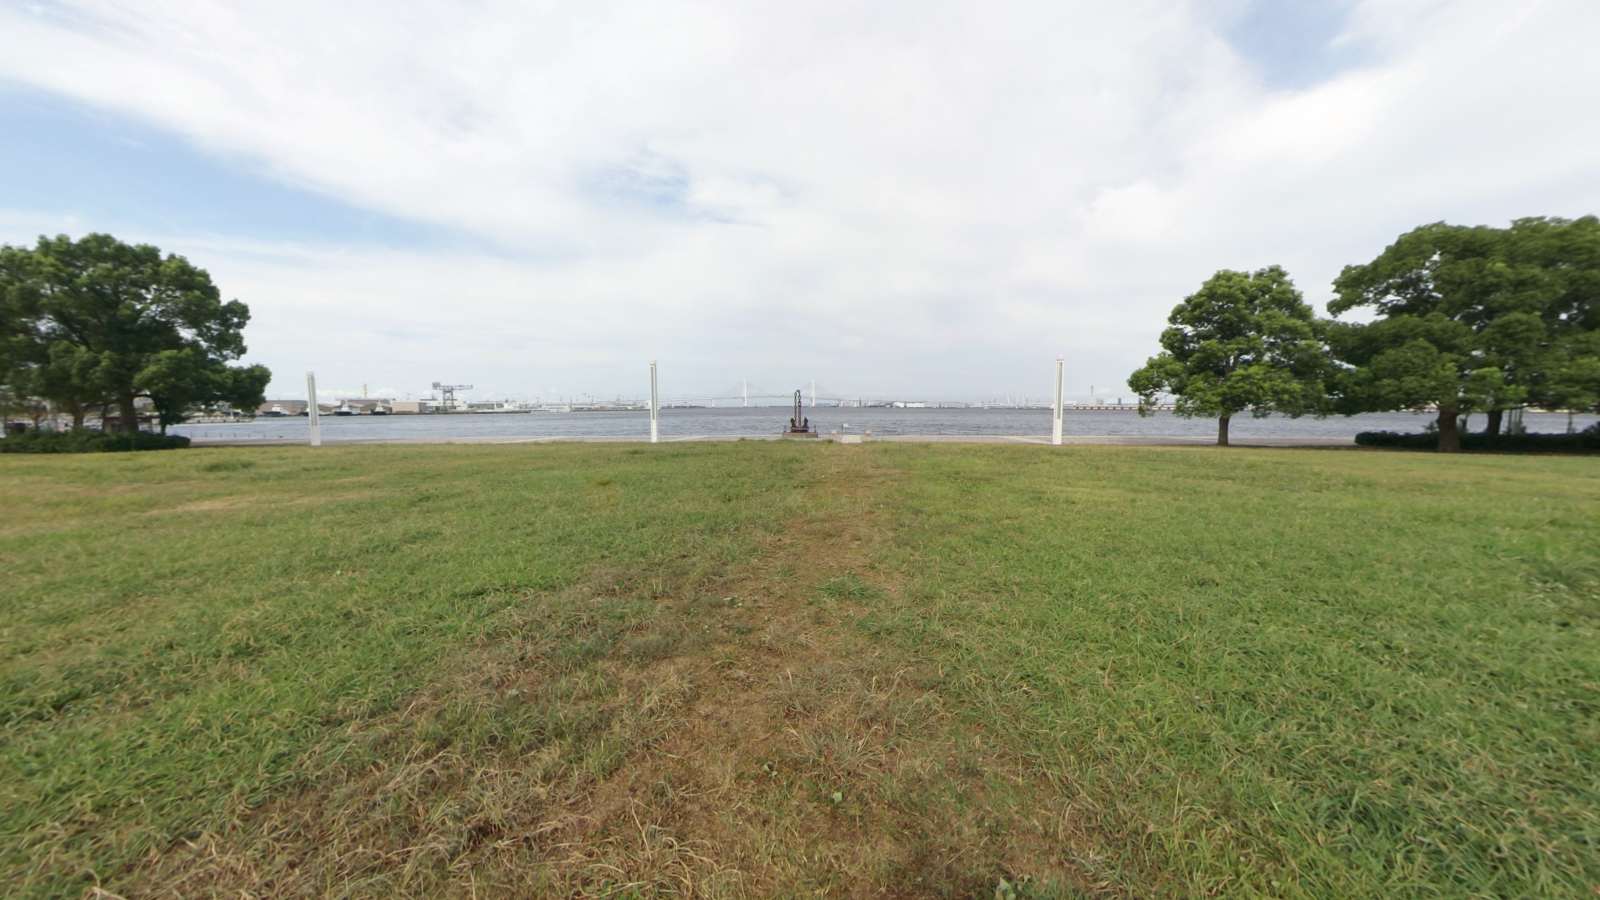
\includegraphics[width=\textwidth]{skybox}

        \href{https://humus.name/index.php?page=Textures&ID=138}{Yokohama2}
        by Emil "Humus" Persson, CC-BY 3.0
    \end{frame}
    \begin{frame}
        \frametitle{Skybox}
        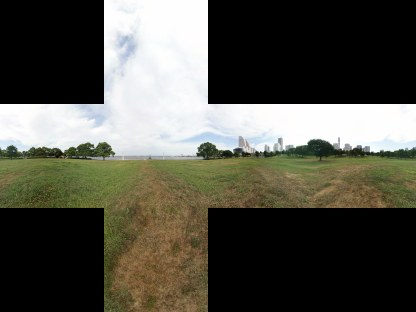
\includegraphics[width=0.8\textwidth]{yokohama2}

        Cubemap texture (6 images, samplerCube) mapped onto a box around origin with radius 1
    \end{frame}
    \begin{frame}[fragile]
        \frametitle{Skybox}
        TF:
        \begin{lstlisting}[language=C++, label={lst:skyboxmvp}]
glm::mat4 TF = VP; // no model
mvp = glm::translate(TF, -cameraPosition);
        \end{lstlisting}
        Vertex shader:
        \begin{lstlisting}[language=glsl,label={lst:skyboxvert}]
gl_Position = TF * vec4(position, 1.0f);
gl_Position = gl_Position.xyww;
uv_out = origin-position;
        \end{lstlisting}
        Fragment Shader:
        \begin{lstlisting}[language=glsl,label={lst:skyboxfrag}]
color.rgba = texture(skybox, uv);
        \end{lstlisting}
    \end{frame}

    \begin{frame}
        \frametitle{Blender objects}

        Disclaimer: I am not good at blender.

        Models generated through normal modeling in blender.

        Basic shading set up to aid intuition

        UV-generation

        Texture-painting directly on model

        Baked normals


    \end{frame}
%    \begin{frame}
%        \frametitle{Object export}
%        Blender can export .obj files (and many other formats)
%
%        Make sure to look properly at all the options (e.g. write normals, triangulate, xyz positive directions)
%
%        You can use a python script to export en masse
%
%        bpy.ops.export\_scene.obj
%
%        Can export smoothed normals
%
%    \end{frame}
%    \begin{frame}
%        \frametitle{Object import}
%
%        I opted to use tinyobjloader here
%
%        Save load time: pretriangulated objects
%
%        (setting in blender and setting in tinyobj call)
%
%        Must generate tangents after load
%
%        Bitangents can be found in shader
%
%    \end{frame}

%    \begin{frame}
%        \frametitle{Blender shading}
%        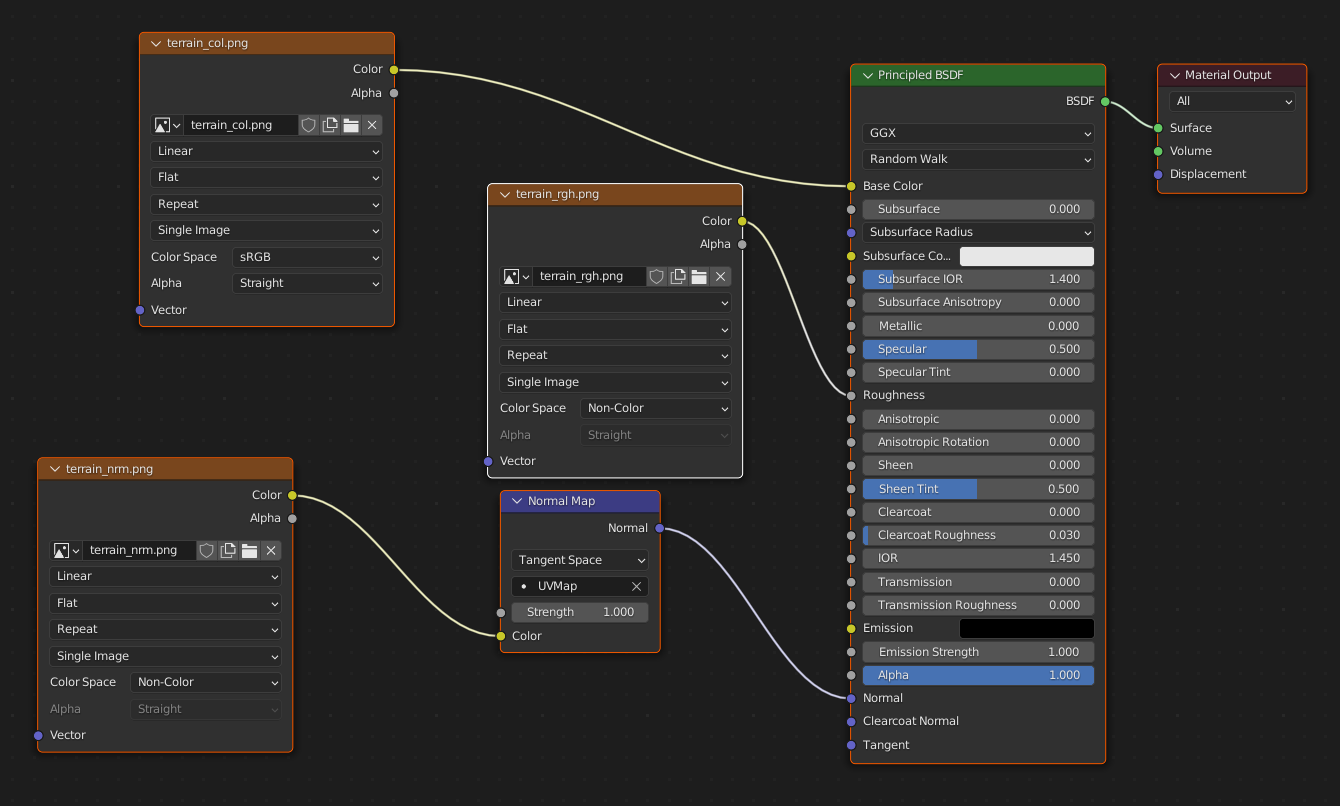
\includegraphics[width=\textwidth]{basicshading}
%    \end{frame}
%    \begin{frame}
%        \frametitle{Trying to preview fur}
%        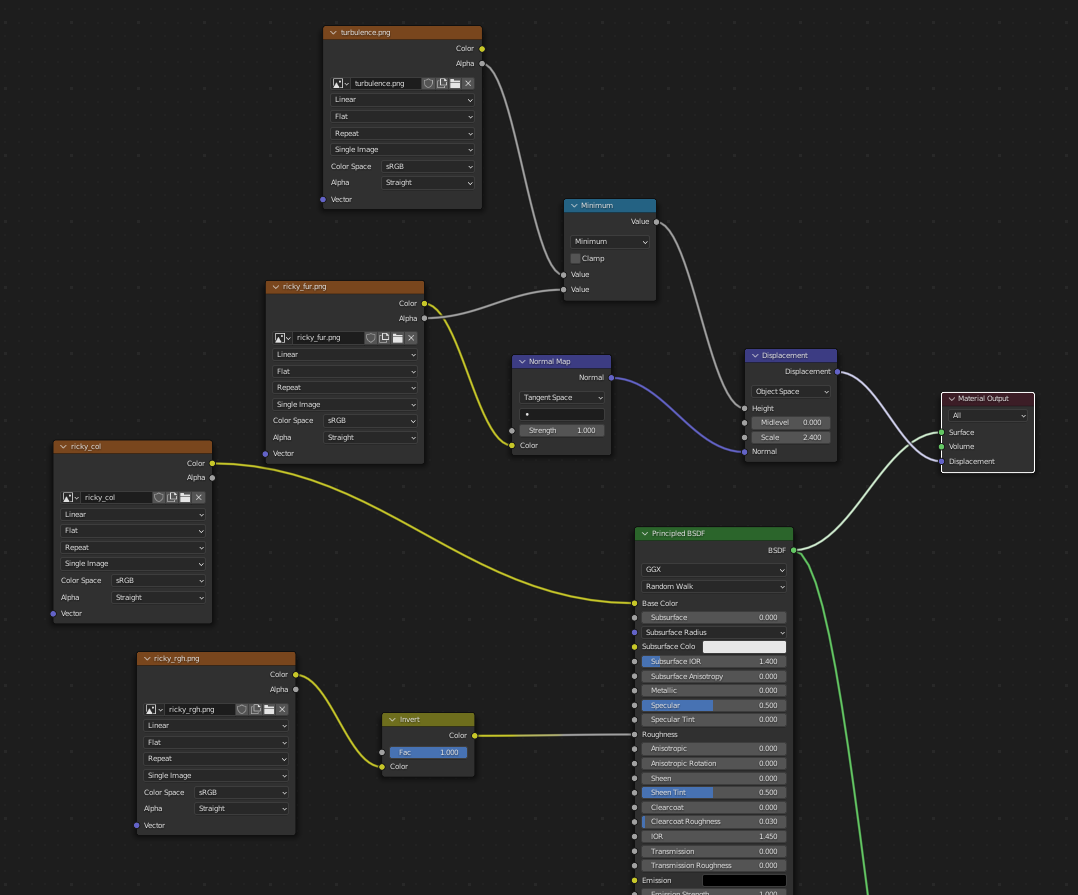
\includegraphics[width=0.8\textwidth]{ohgodshading}
%    \end{frame}
    \begin{frame}
        \frametitle{Trying to preview fur ...Wasn't super helpful}
        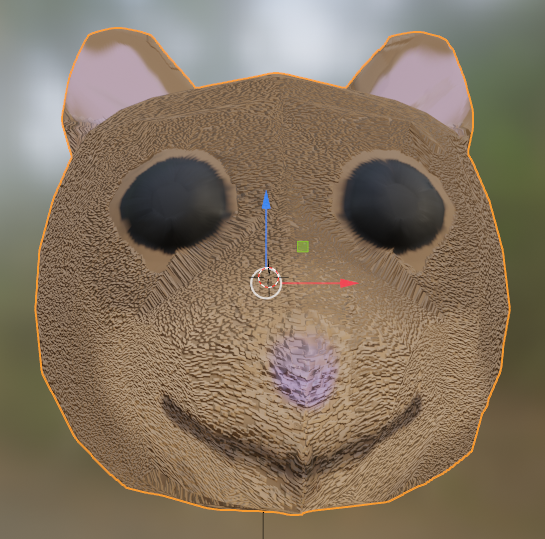
\includegraphics[width=0.8\textwidth]{roughricky}
    \end{frame}
    \begin{frame}
        \frametitle{ UVs are annoying, huh?}
        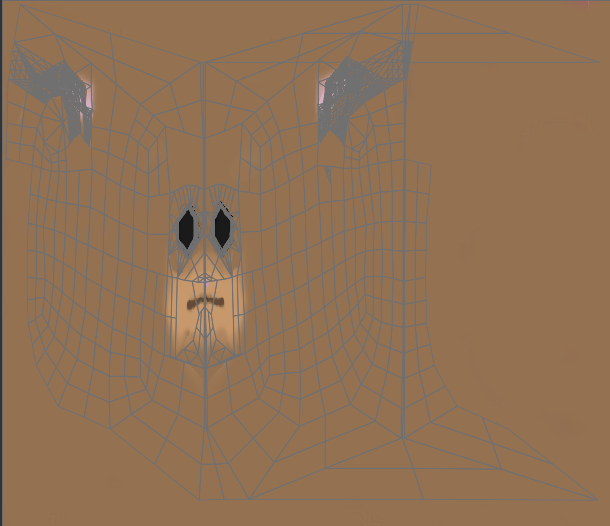
\includegraphics[width=0.7\textwidth]{UVs}
    \end{frame}
    \begin{frame}
        \frametitle{ ...I messed up the ear area}
        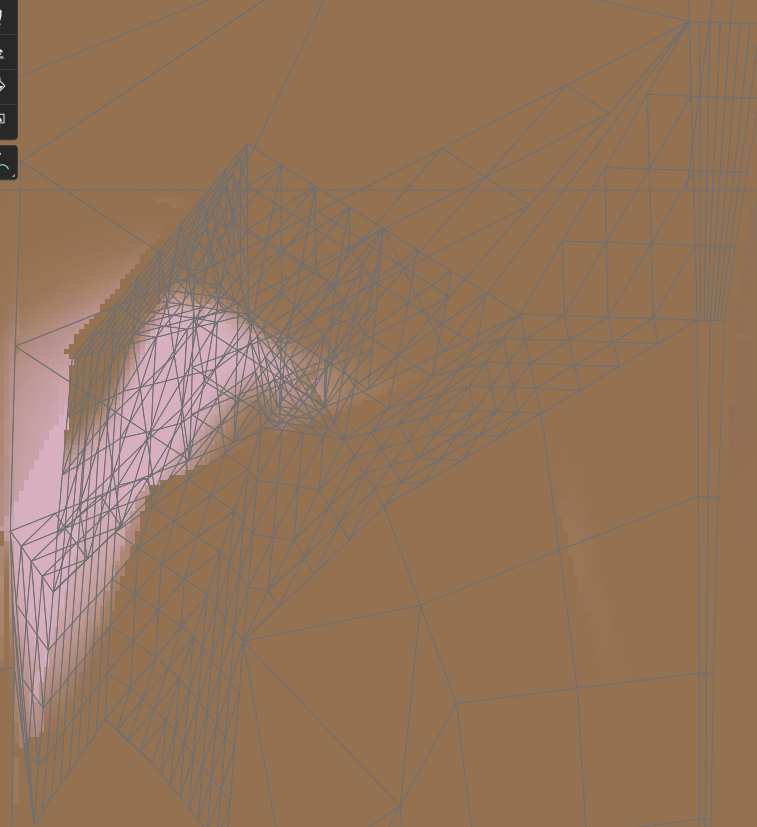
\includegraphics[width=0.7\textwidth]{overlapUVs}
    \end{frame}
%    \begin{frame}
%        \frametitle{ Texture painting}
%        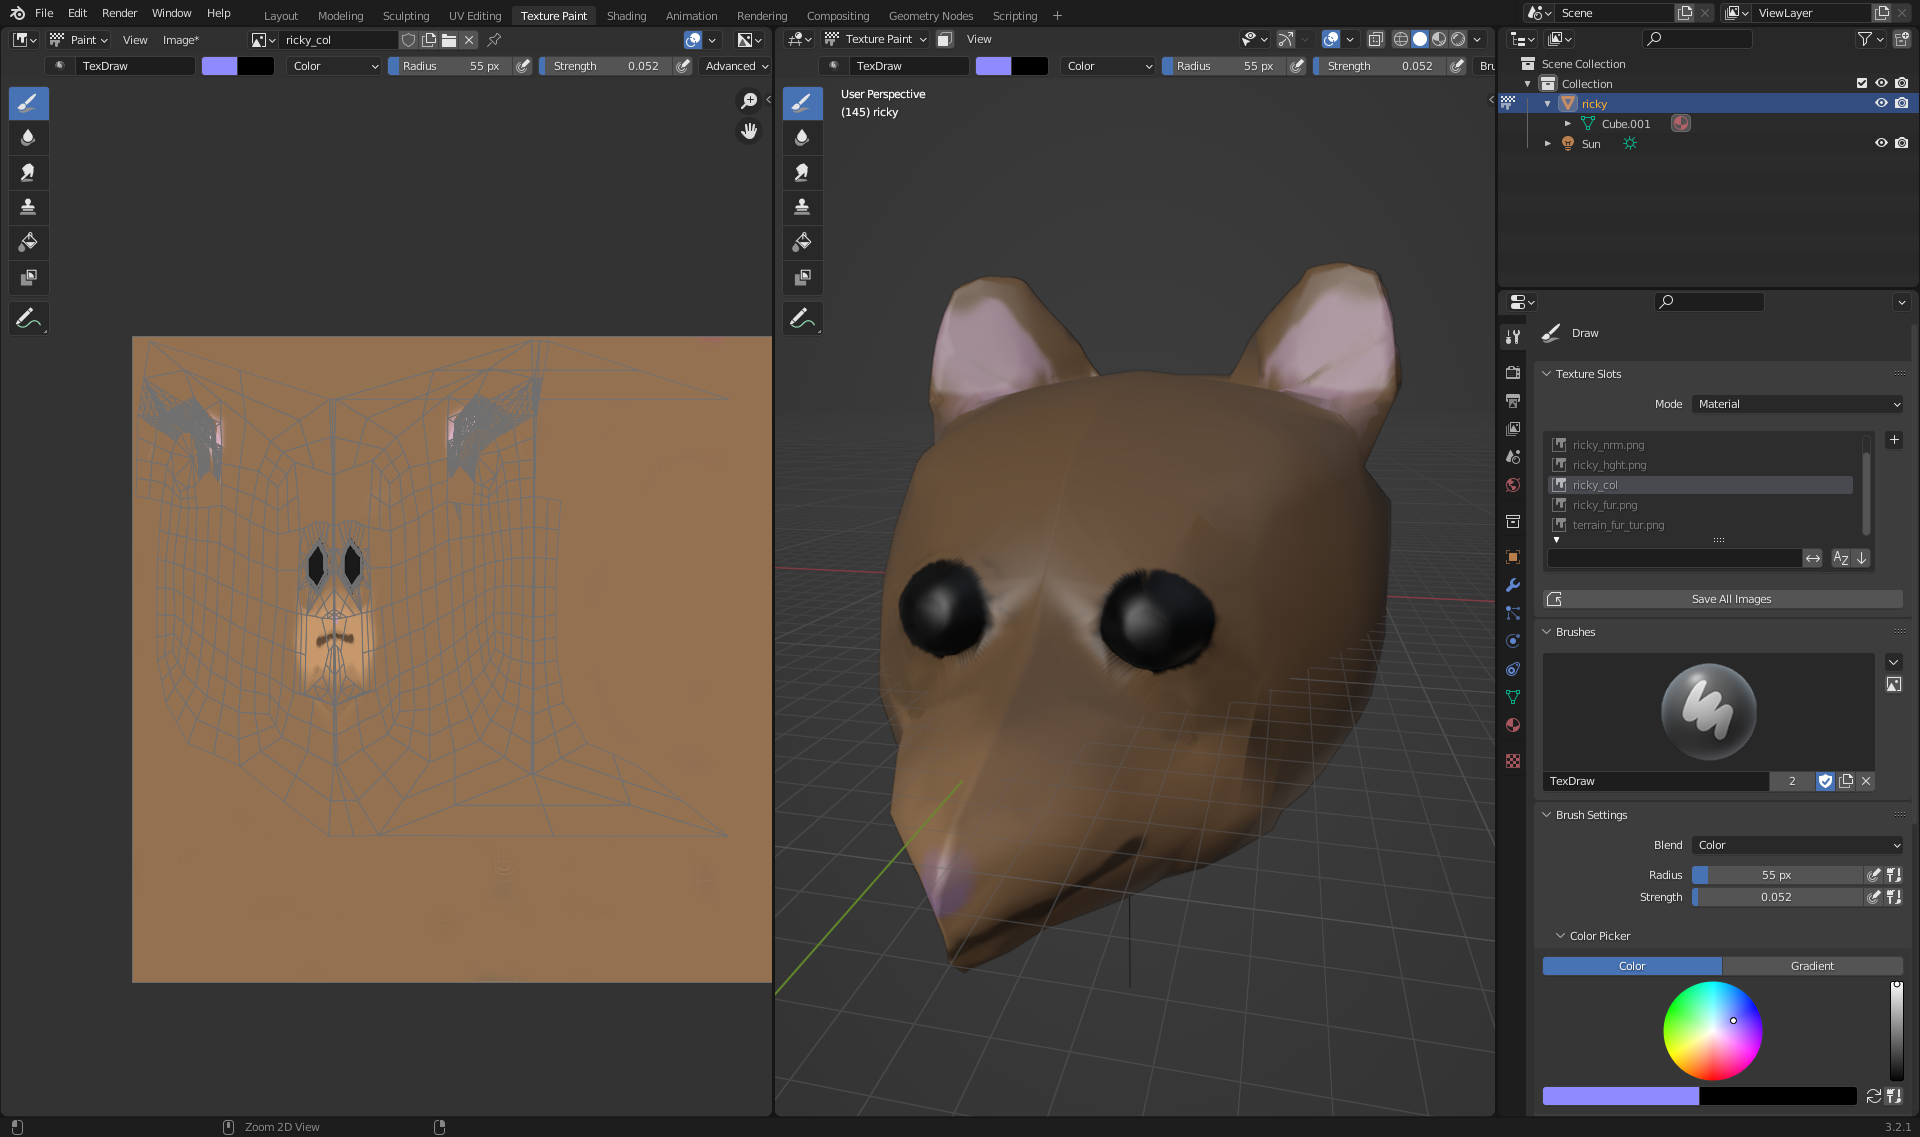
\includegraphics[width=\textwidth]{texturepaint}
%    \end{frame}
    \begin{frame}
        \frametitle{ Texture painting}
        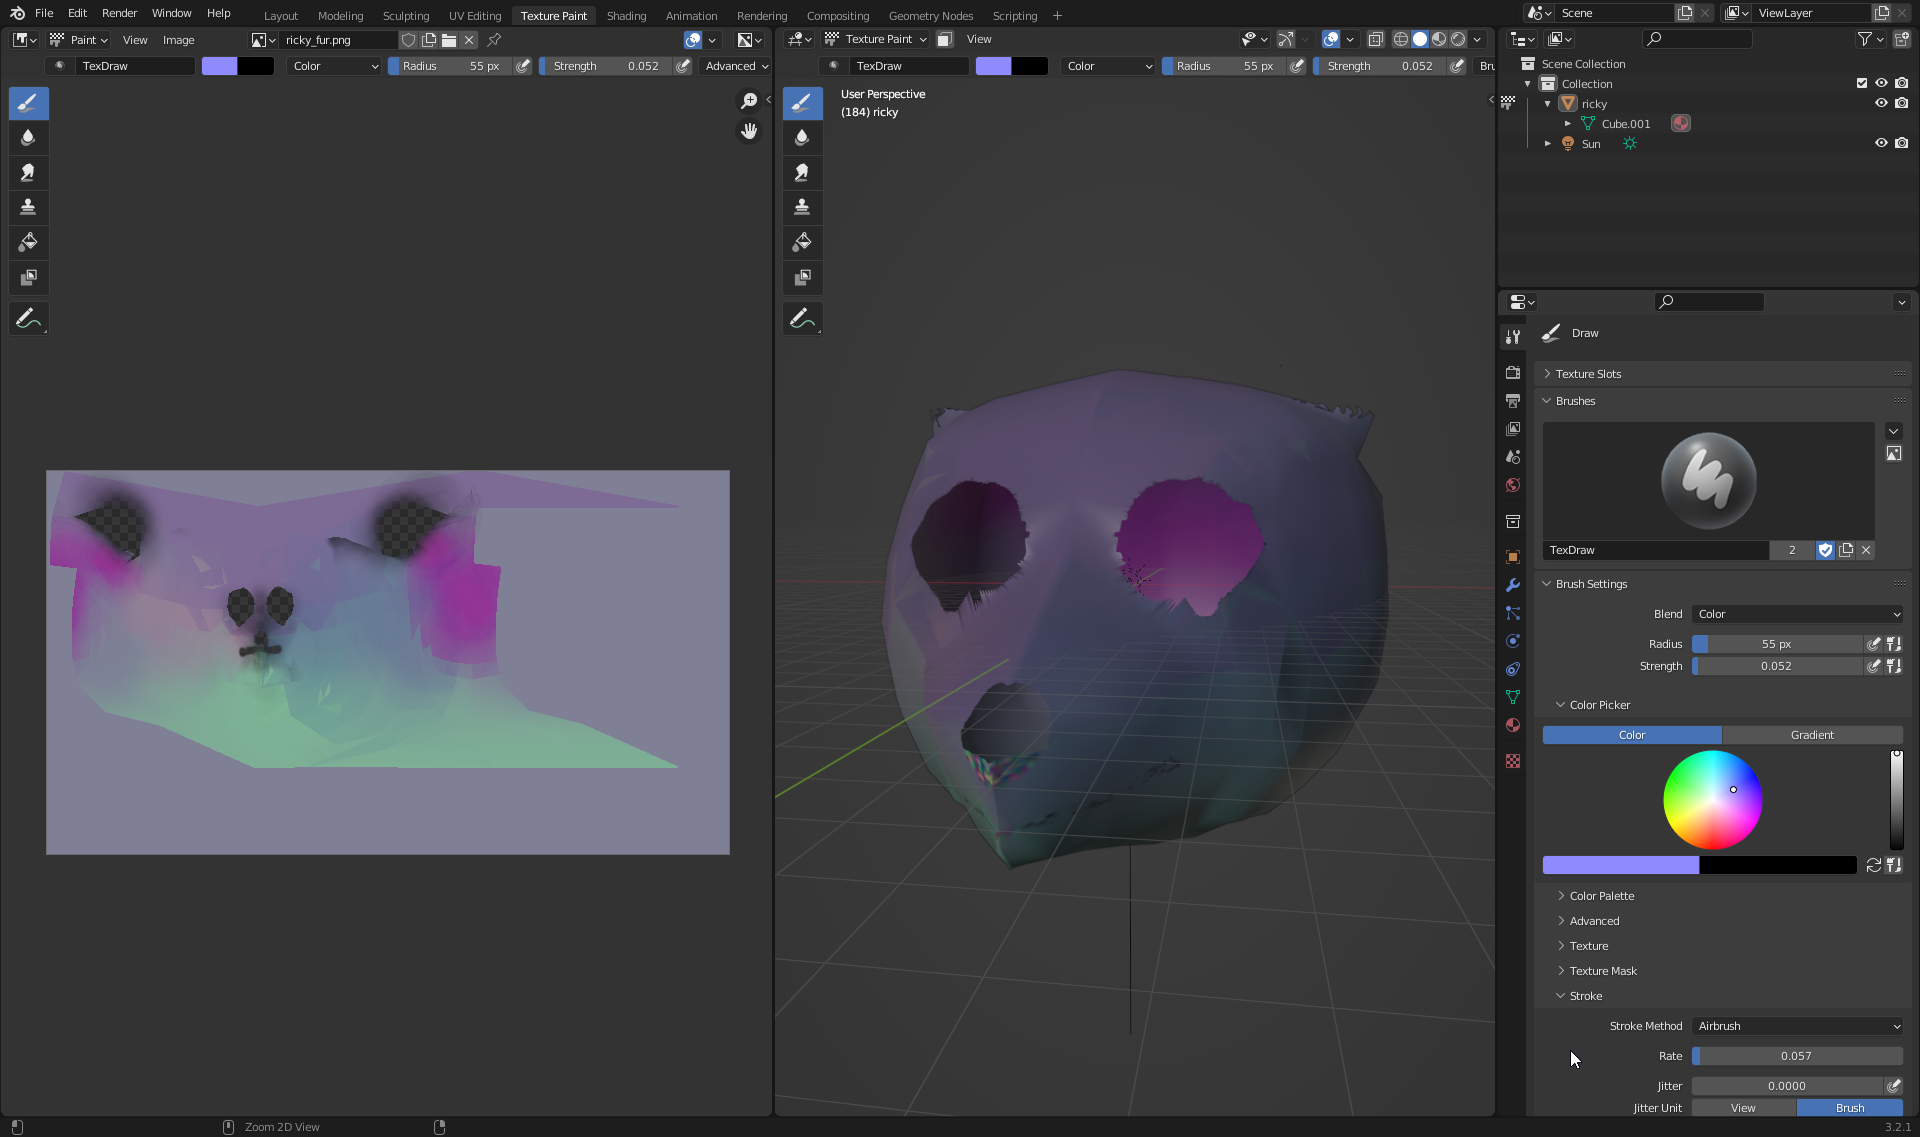
\includegraphics[width=\textwidth]{texturepaint2}
    \end{frame}
    \begin{frame}
        \frametitle{ displacement map baked normals }
%        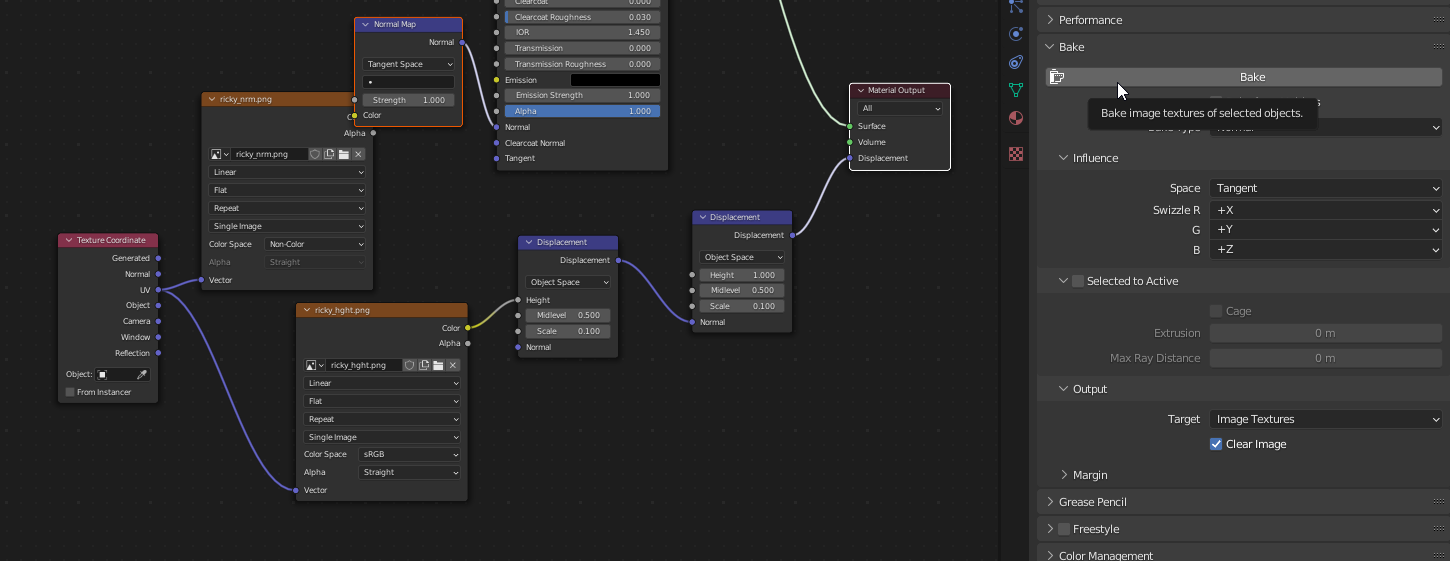
\includegraphics[width=\textwidth]{bake}
%    \end{frame}
%    \begin{frame}
%        \frametitle{ Result }
        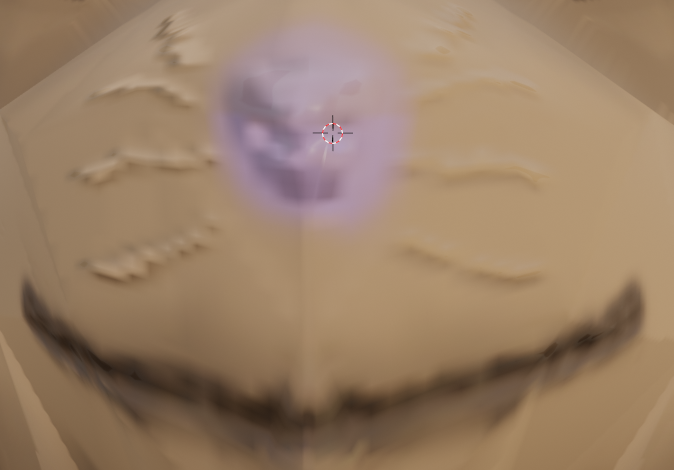
\includegraphics[width=\textwidth]{nosewhiskers}
    \end{frame}

    \begin{frame}
        \frametitle{ Shell method fur generation }

        Render solid base

        Render shells with geometry shader

        Triangle $\rightarrow$ several displaced copies

        Texture lookup determines direction and length of displacement

        A uniform also scales displacement
        
        Can add uniform vector for further dynamic displacement (wind, interaction)
        
    \end{frame}
    
    \begin{frame}
        \frametitle{ Forming Strands }
        Render mostly transparent shells, with 'dots' of visibility.

        These dots form lines, strands of fur.

        Darker roots, brighter tips, for cheap 'self-shadowing'

        'Thinning' through lowering alpha along length.

        Could use 3D textures
        \vspace{0.5em}

        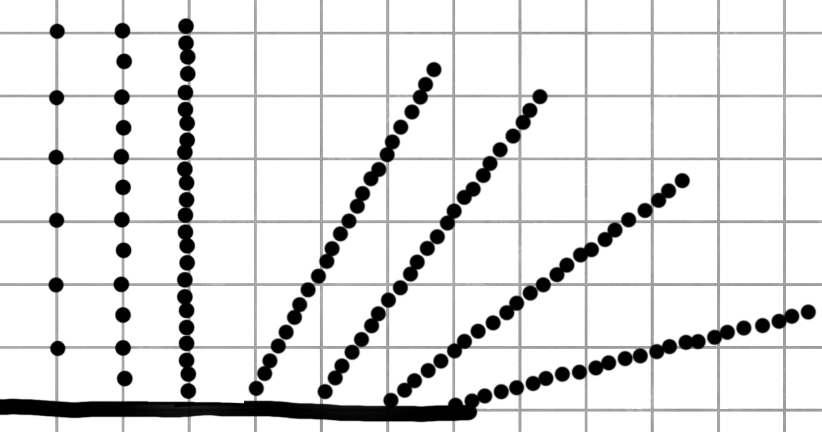
\includegraphics[width=0.7\textwidth]{dotsformlines}
    \end{frame}

    \begin{frame}
        \frametitle{ Shell result: }

        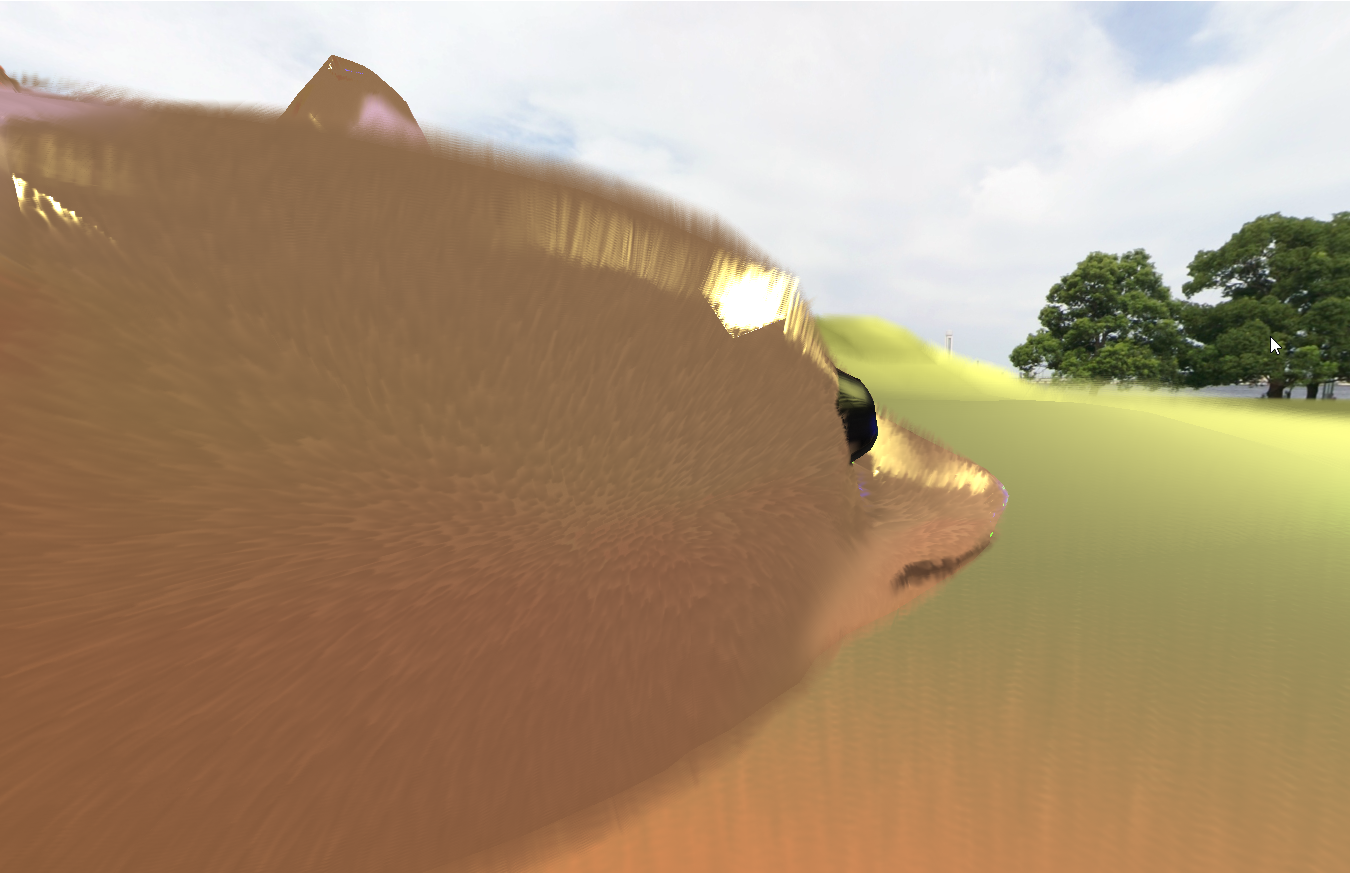
\includegraphics[width=\textwidth]{shells}
    \end{frame}

    \begin{frame}
        \frametitle{ Dots texture: }

        Dots are stored as a texture,

        generated with a simple python script.

        Could replace this with 3d texture,

        Could scale UVs (density uniform?)

        to loop faster than other textures to save on space

        Could make it implicit with some function in shaders

        Could rig it to be more localized
    \end{frame}

    \begin{frame}
        \frametitle{ Downside }

        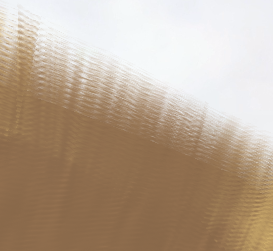
\includegraphics[width=12em]{shellgaps}
    \end{frame}

    \begin{frame}
        \frametitle{ Fin method fur generation}
        Dynamically generate fur cards

        (Billboards that show fur strands)

        Helps cover the silhouette,

        where you see between the layers of the shells better

        This is also done with a geometry shader
    \end{frame}

    \begin{frame}
        \frametitle{ Fin method fur generation}

        Idea: edge $\rightarrow$ billboard

        NVIDIA: adjacent triangles $\rightarrow$ billboard

        My solution: triangle $\rightarrow$ 3 billboards (as triangle-strips)

        Only edges at/near silhouette

        Fade in and out

        Draw if camera-to-point is near-normal on edge-normals.

        Billboards follow fur direction away from original edge

        Density determined by edge density

        Segmented vertically to enable 3d effects (like bending nonlinearly in wind)

    \end{frame}

    \begin{frame}
        \frametitle{ Fin Method results }
        Fins do not easily sell volume
        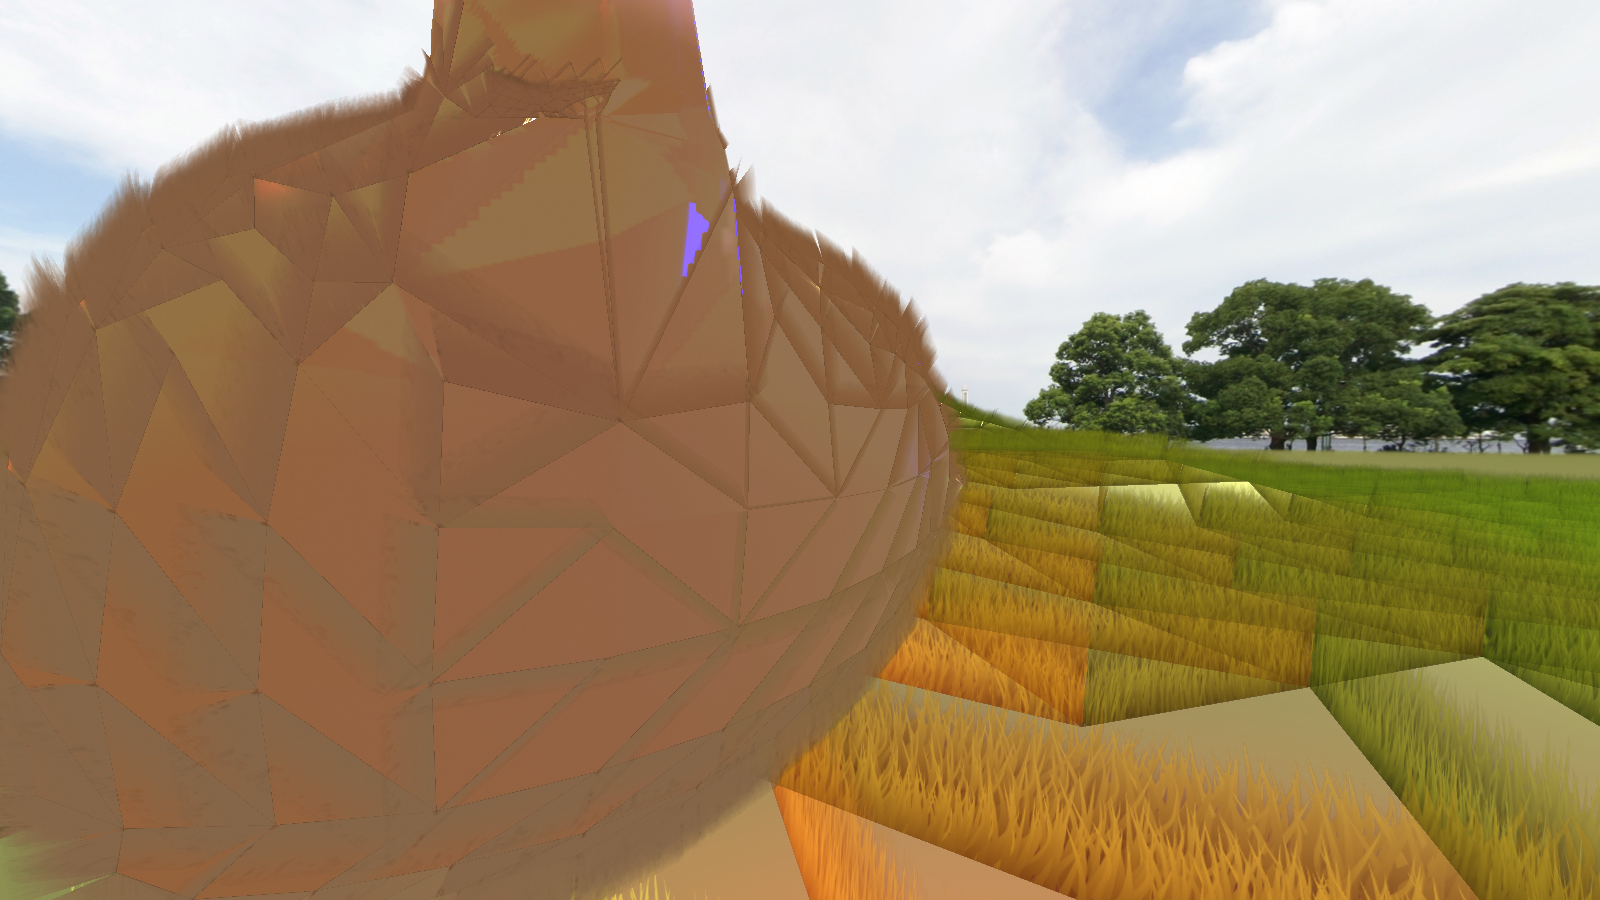
\includegraphics[width=\textwidth]{fullfins}
    \end{frame}
    \begin{frame}
        \frametitle{ Fin Method results }
        They do work great at the silhouette though
        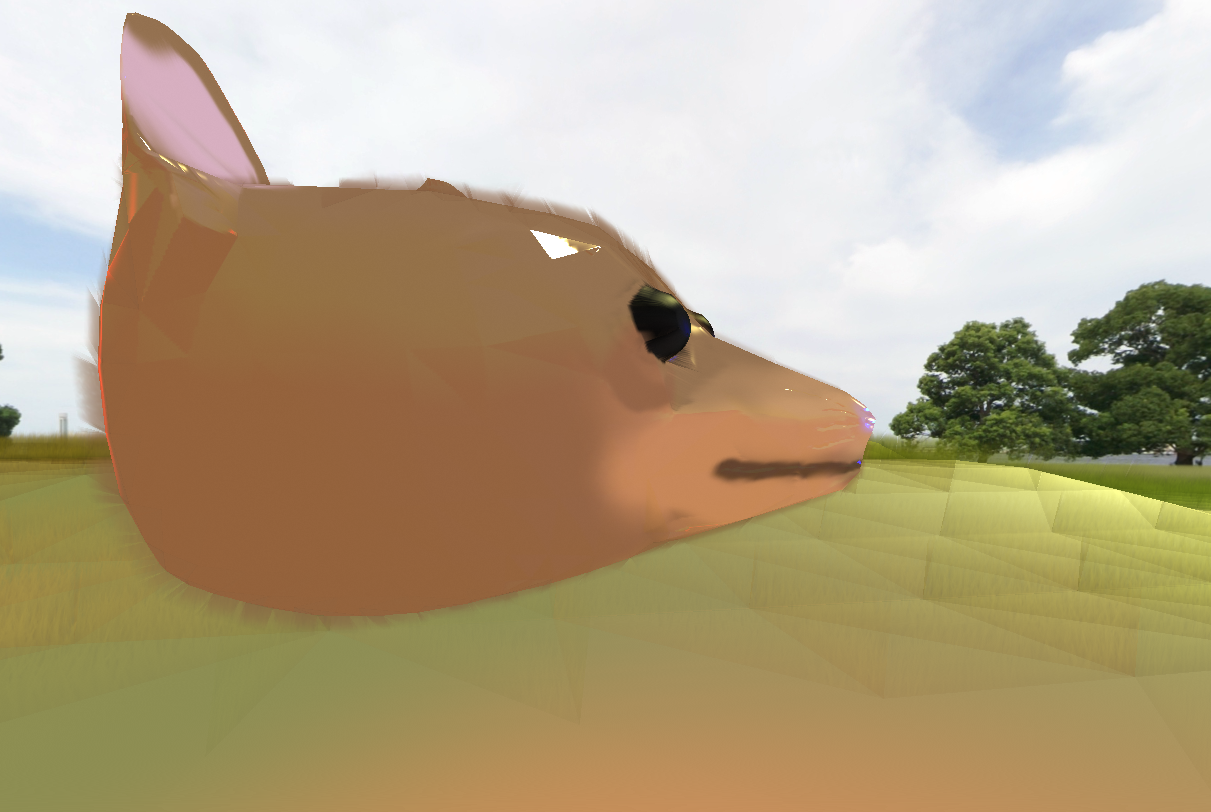
\includegraphics[width=\textwidth]{fins}
    \end{frame}
    \begin{frame}
        \frametitle{ Fins textures }
        The grass texture was found free online
        https://pixabay.com/vectors/grass-background-border-green-grass-2029768/

        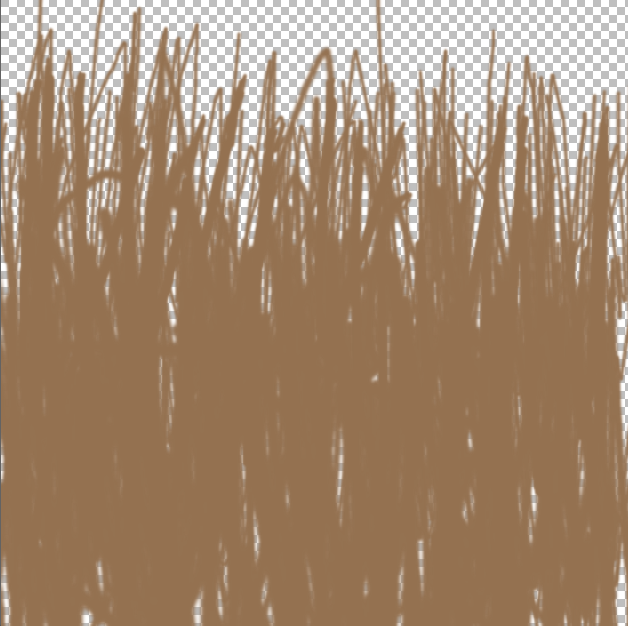
\includegraphics[width=0.5\textwidth]{rickystrands}%
        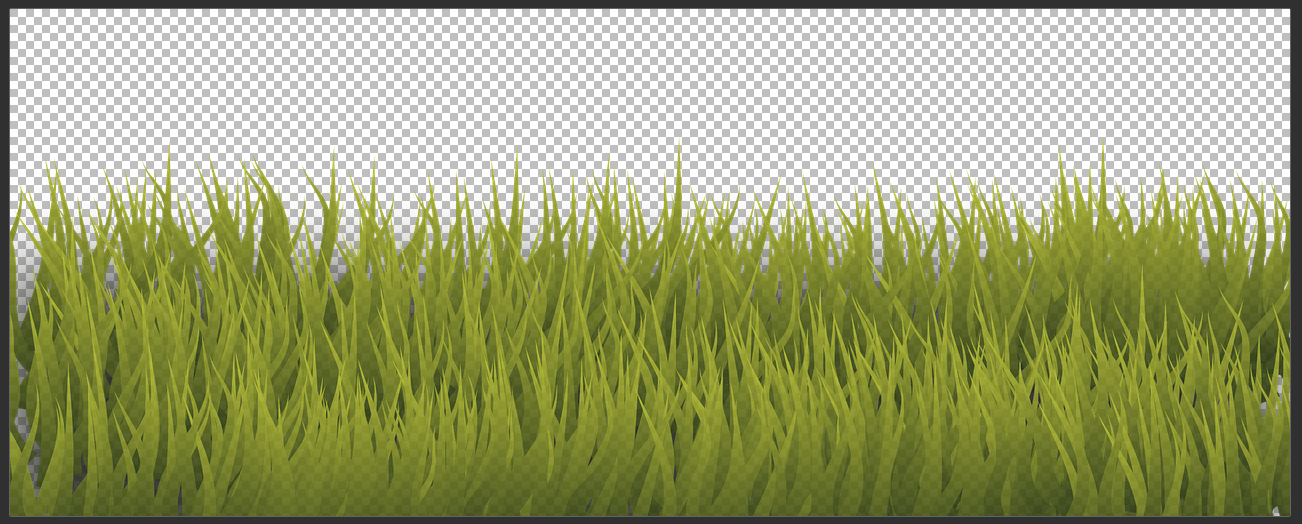
\includegraphics[width=0.5\textwidth]{terrainstrands}
    \end{frame}

    \begin{frame}
        \frametitle{Blending}

        Hair and fur notably have very fine detail

        My methods uses a lot of alpha.

        Hard to depth-sort volumes and billboards?

        Lots of self-occlusion
    \end{frame}

    \begin{frame}
        \frametitle{Self-occlusion}

        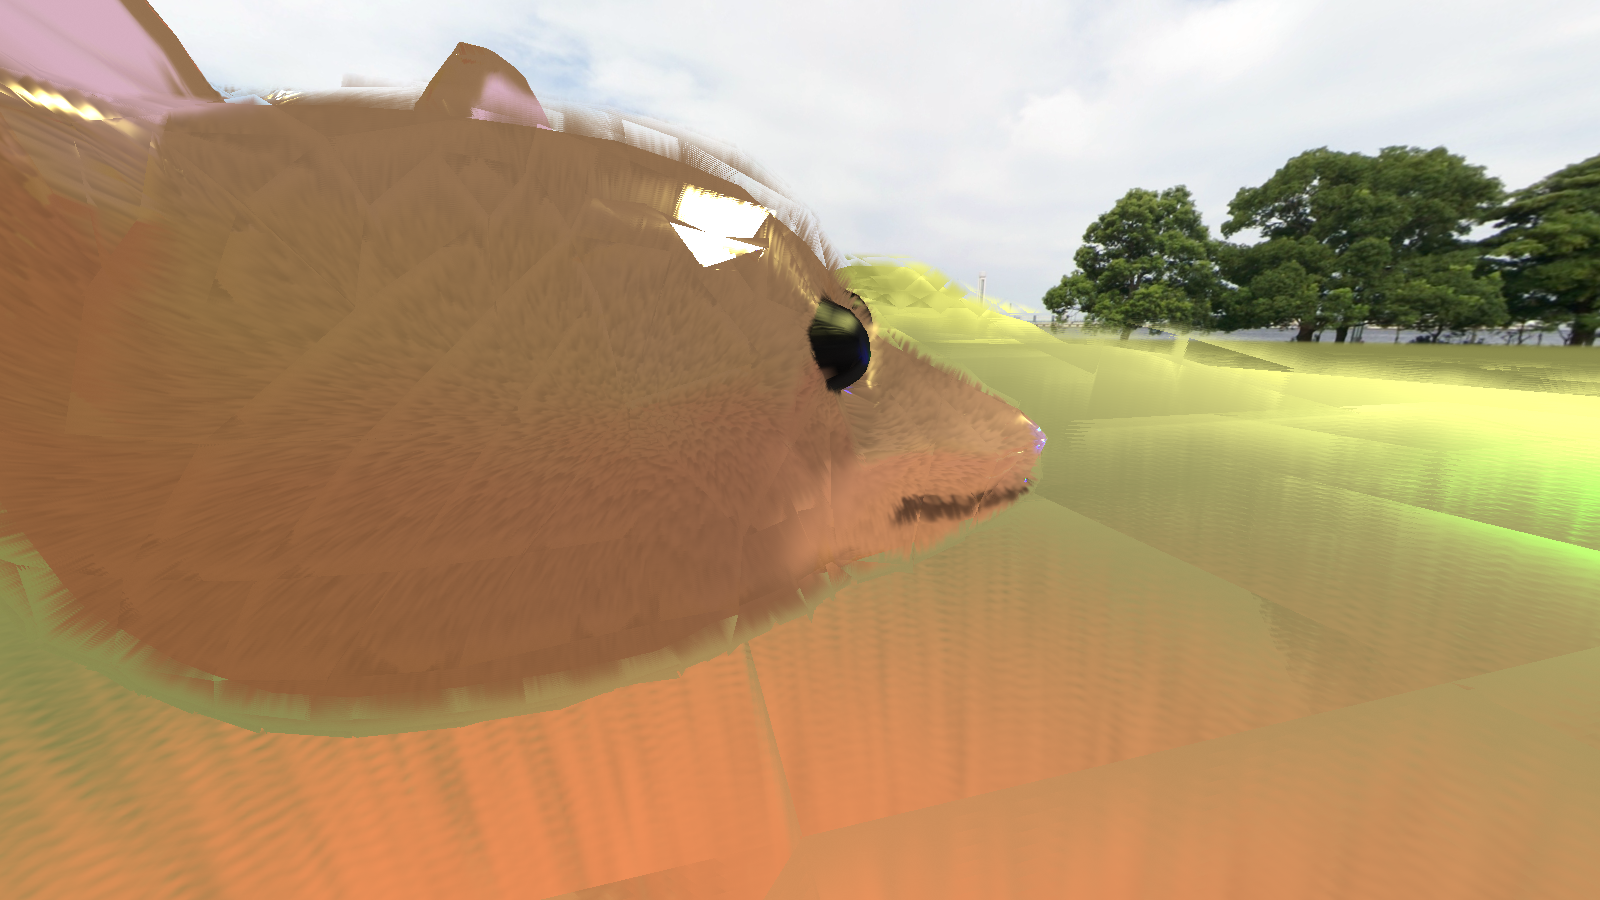
\includegraphics[width=\textwidth]{selfocclusiongalore}
    \end{frame}
    \begin{frame}
        \frametitle{No depth mask}

        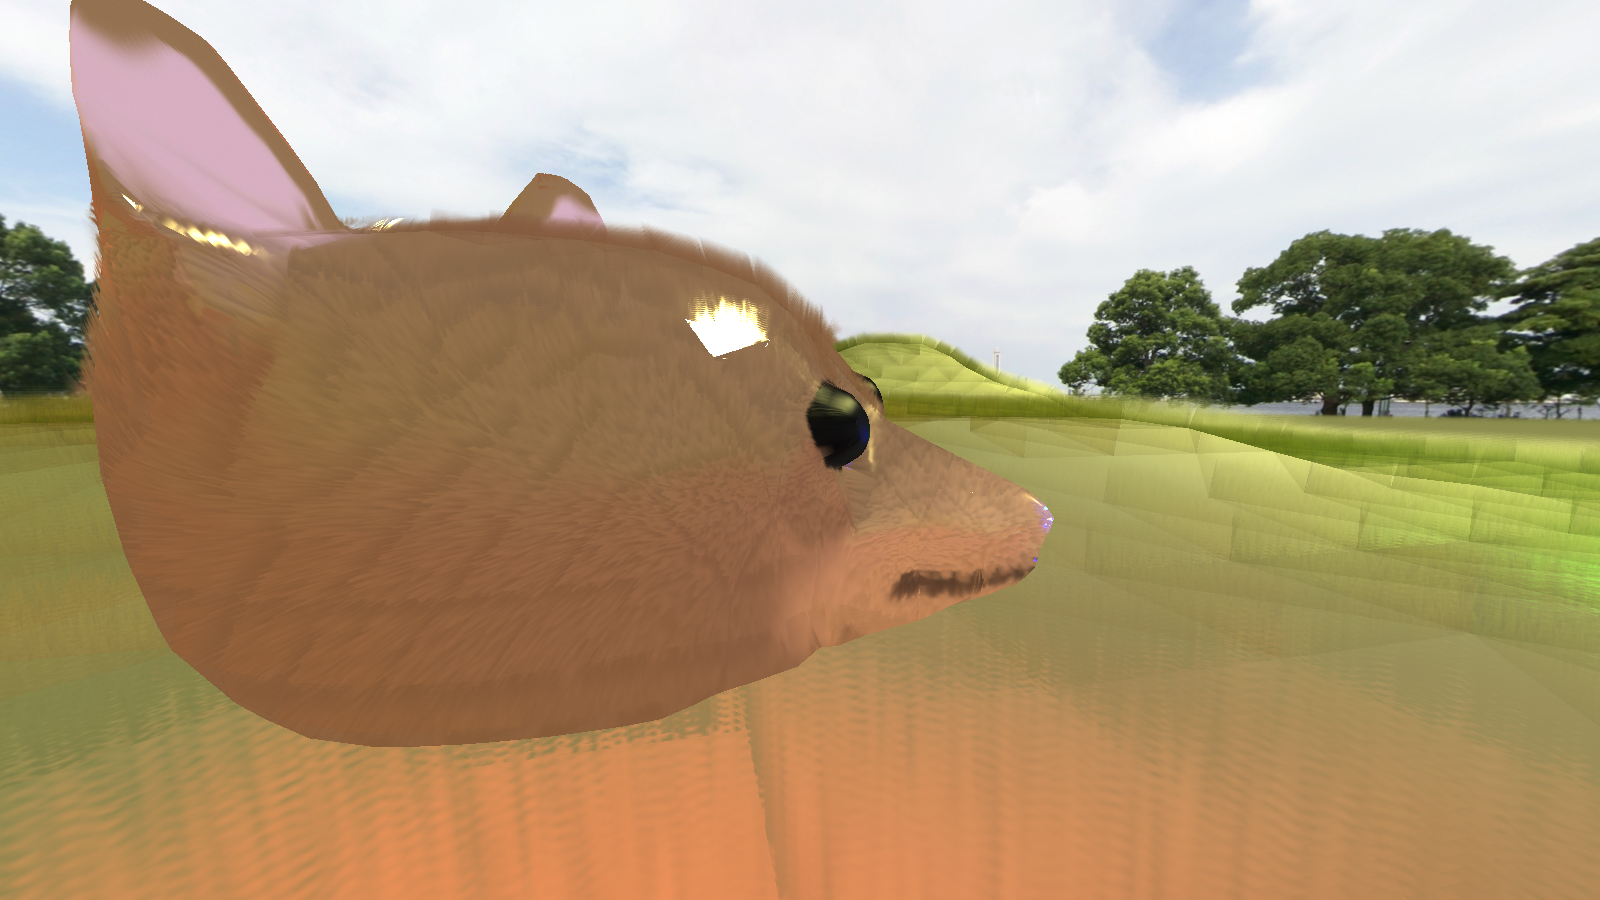
\includegraphics[width=\textwidth]{selfoccnodepthmask}
    \end{frame}

    \begin{frame}
        \frametitle{Weighted Blended Order-Independent Transparency}

        Multipass multichannel method.

        \begin{enumerate}
            \item Render Opaque Elements (skybox, bases)
            \item Semitransparent render
            \begin{enumerate}
                \item Occlude base color from background \\ (colored glass filtering) (optional)
                \item Add lit color to accumulation buffer \\ (depth and alpha weighted contribution)
                \item Add weight to accumulation buffer alpha
                \item Lower revealage (remaining transparency) \\by original alpha
            \end{enumerate}
            \item Composite accumulation-buffer onto image
            \begin{itemize}
                \item divide by accumulation-alpha to scale the average
                \item alpha of composite layer = 1 - revealage
            \end{itemize}
        \end{enumerate}
    \end{frame}

    \begin{frame}
        \frametitle{Blending results}
        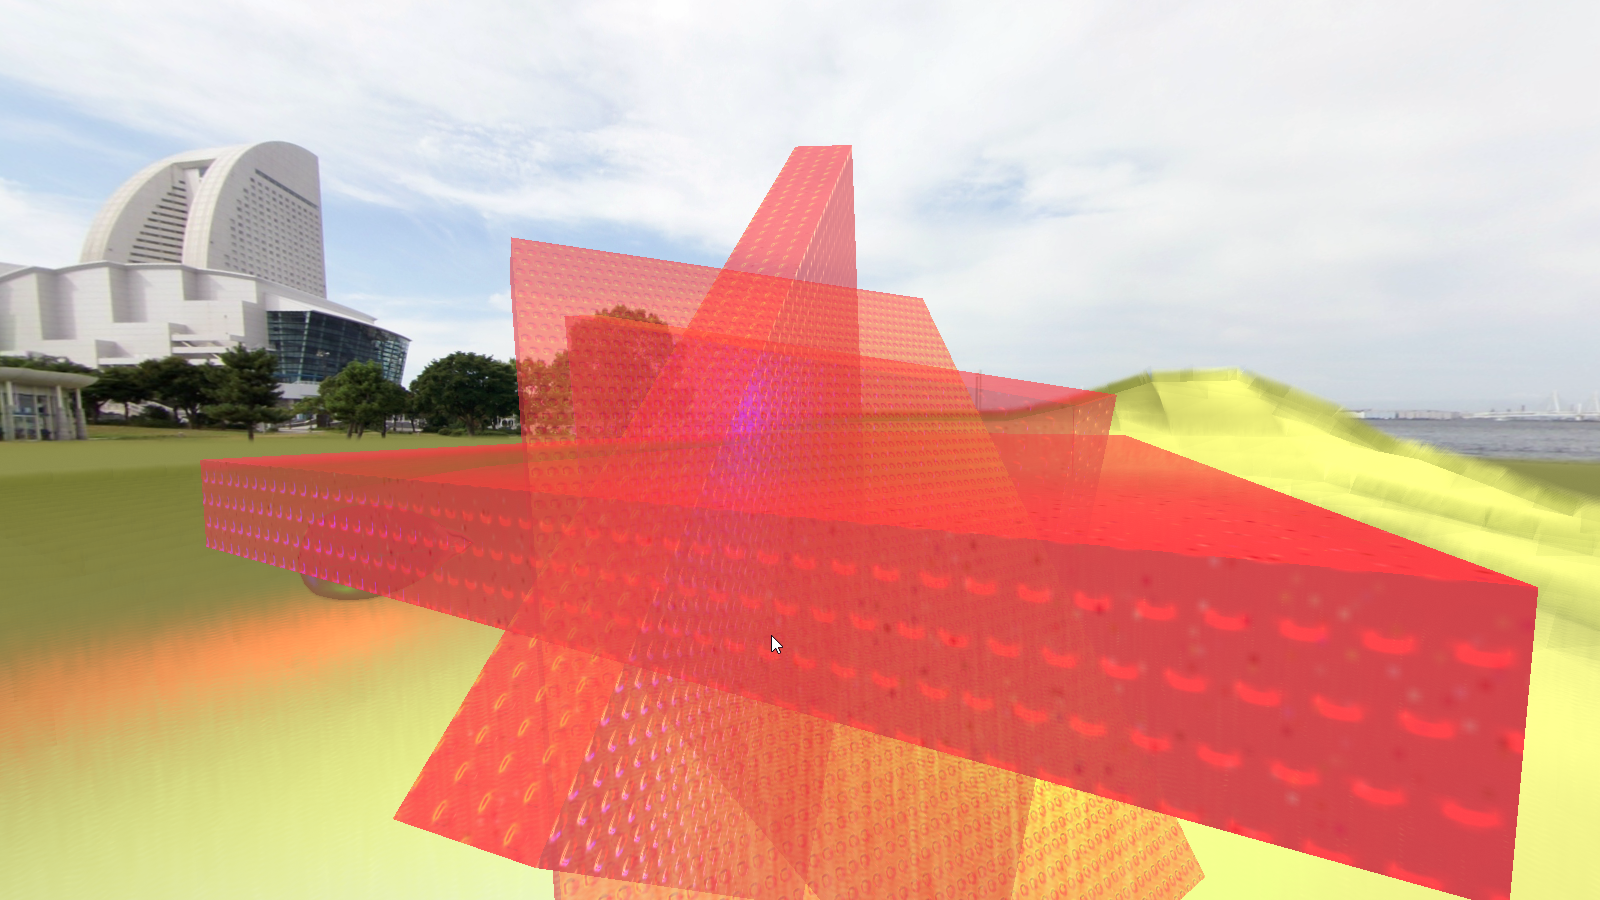
\includegraphics[width=\textwidth]{blending}
    \end{frame}

\end{document}